\documentclass[class=IEEEtran]{standalone}%[conference,10pt]{IEEEtran}
\usepackage{amsmath}
\ifCLASSINFOpdf
\usepackage[pdftex]{graphicx}
\else
\usepackage[dvips]{graphicx}
\fi

\usepackage{color}	% required for `\textcolor' (yatex added)

%ERIC ADDED:
\usepackage{xcolor, tikz, pgfplots, ifthen}
\usepackage[american,cuteinductors,smartlabels]{circuitikz}
\pgfplotsset{compat=newest}
\usetikzlibrary{intersections,calc,backgrounds}

\begin{document}
	
	
	\centering
	
	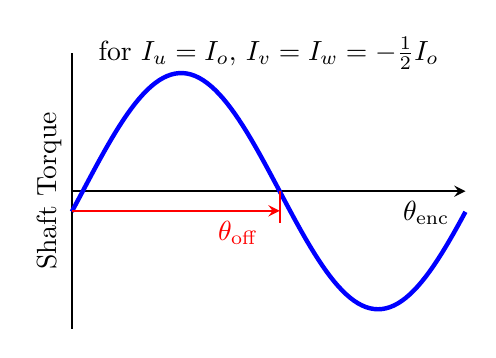
\begin{tikzpicture}[>=stealth]
		% Axes
		\draw[thick, ->] (0,0) -- (5,0) node[anchor=west, below, pos=0.9] {$\theta_{\rm enc}$};
		\draw[thick] (0,-1.75) -- (0,1.75) node[anchor=south, rotate = 90, pos = 0.5] {Shaft Torque};
		
		% Blue sinusoidal curve
		\draw[blue, ultra thick, domain=0:5, samples=100] plot (\x, {1.5*sin(360*\x/5 - 10)});
		
		% Red arrow and label
		\draw[red, thick, ->] (0,-.25) -- (2.64,-.25) node[pos = 0.8, anchor=north] {$\theta_{\rm off}$};
		\draw[red, thick] (2.64, -.4) -- (2.64, 0);
		
		% Text at the top
		\node at (2.5,1.75) {for $I_u = I_o$, $I_v = I_w = -\frac{1}{2} I_o$};
	\end{tikzpicture}
\end{document}

